\documentclass[a4paper]{article}

% subfile handling packages
\usepackage{subfiles}
\newcommand{\onlyinsubfile}[1]{#1}
\newcommand{\notinsubfile}[1]{}

% document packages
\usepackage[top=1in, bottom=1.25in, left=1.25in, right=1.25in]{geometry}
\usepackage{amsmath}
\usepackage{multicol}
\usepackage{graphicx}
\RequirePackage{ltxcmds}[2010/12/07]
\graphicspath{{../../images/}}
%\graphicspath
\usepackage{float}
\usepackage{amsfonts}

% Document metadata
\title{BPSK system}
\author{ }
\date{ }

\begin{document}
\renewcommand{\onlyinsubfile}[1]{}
\renewcommand{\notinsubfile}[1]{#1}

\maketitle

\section{Introduction}

This document describes the simulation BPSK system in back-to-back configuration. 

\section{Functional Description}

A simplified diagram of the system being simulated is presented in the Figure~\ref{fig:physicalsystem}. The system simulated takes a random binary string and encodes it in an optical bandpass signal, signal that afterwards is decoded in order to re-obtain the original binary string.
\par
The decoding of the optical signal is accomplished by an homodyne receiver, which combines the signal with a local oscillator with a user-determined phase. The homodyne receiver block output is then fed into a block that compares it with the original binary string and computes the Bit Error Rate (BER) along with it's upper and lower bounds for a certain user defined confidence level.

\begin{figure}[h]
\centering
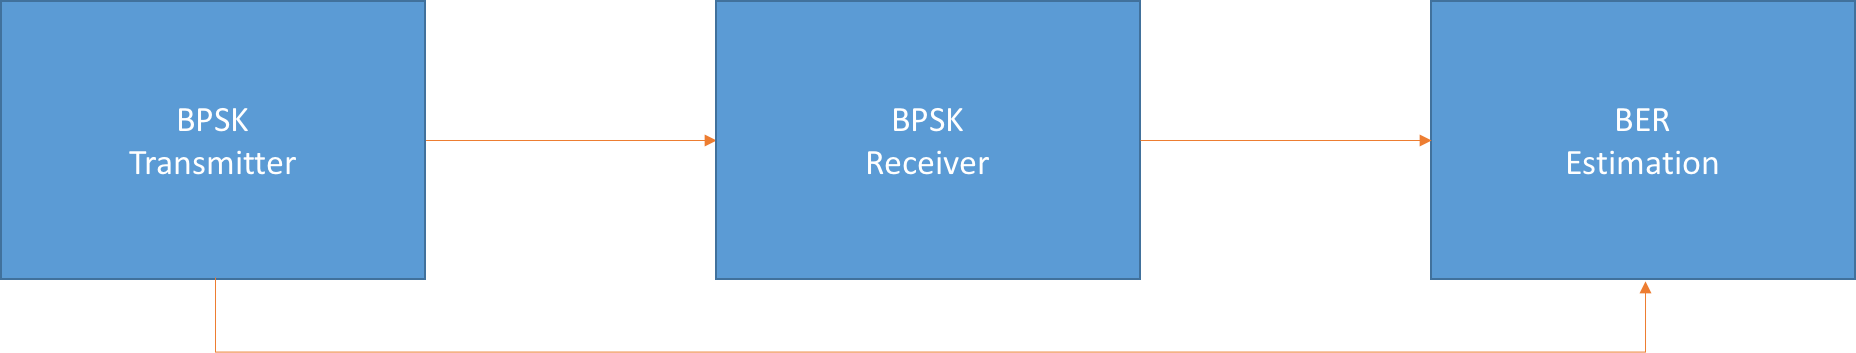
\includegraphics[width=\linewidth]{bpskdiagram.png}
\caption{Overview of the BPSK system being simulated.}
\label{fig:physicalsystem}
\end{figure}

\begin{table}[H]
\centering
\begin{tabular}{c|c}
System Blocks    & netxpto Blocks   \\ \hline
BPSK Transmitter & MQamTransmitter  \\
BPSK Receiver    & HomodyneReceiver \\
BER Estimator    & BitErrorRate                      
\end{tabular}
\end{table}

\section{System Input Parameters}

This system takes into account the following input parameters:

\begin{table}[H]
\centering
\begin{tabular}{c|c}
System Parameters    			 & netxpto Parameters     \\ \hline
Length of Binary String 			 & NumberOfBits           \\
Number of Samples per Bit 		 & SamplesPerSymbol       \\
Binary String Pattern Length 	 & pLength                \\
Constellation 					 & iqAmplitudesValues     \\
Signal Optical Power 			 & outOpticalPower\_dBm   \\
Local Oscillator Optical Power	 & LOoutOpticalPower\_dBm \\
Local Oscillator Phase 			 & LocalOscillatorPhase   \\
Beam Splitter Transfer Matrix 	 & TransferMatrix         \\
Photodiode Responsivity 			 & Responsivity           \\
Amplification Factor 			 & Amplification          \\
Amplitude of Thermal Noise        & NoiseAmplitude         \\
Number of Samples to be discarded & Delay                  
\end{tabular}
\end{table}

\section{Inputs}

This system takes no inputs.

\section{Outputs}

This system outputs the following objects:
\begin{itemize}
\item Signals:
\begin{itemize}
\item Initial Binary String; (MQAM$_0$)
\item Optical Signal with coded Binary String; (S$_{00}$)
\item Decoded Binary String; (S$_{01}$)
\end{itemize}
\item Other:
\begin{itemize}
\item Bit Error Rate report in the form of a .txt file. (BER.txt)
\end{itemize}
\end{itemize}

\section{Simulation Results}

We consider the following scenarios:
\begin{itemize}
\item \ref{subsec:scenario1} Basic BPSK back to back with normally distributed thermal noise.
\end{itemize}

\subsection{BPSK with thermal noise}\label{subsec:scenario1}

The following results were obtained from the simulation using the following input parameters:
\begin{table}[H]
\centering
\begin{tabular}{rl}
NumberOfBits=           & 1000                                                     \\
SamplesPerSymbol=       & 16                                                       \\
pLength=                & 5                                                        \\
iqAmplitudesValues=     & \{ \{ 1, 0 \}, \{ -1, 0 \} \}                            \\
outOpticalPower\_dBm=   & -20                                                      \\
LOoutOpticalPower\_dBm= & -10                                                      \\
LocalOscillatorPhase=   & 0                                                        \\
TransferMatrix=         & \{ \{ 1/sqrt(2), 1/sqrt(2), 1/sqrt(2), -1/sqrt(2) \} \}  \\
Responsivity=           & 1                                                        \\
Amplification=          & 1e6                                                      \\
NoiseAmplitude=         & 15.397586549153788                                       \\
Delay=                  & 9                                                        \\
\end{tabular}
\end{table}

The system took the binary string presented in Figure~\ref{fig:sentkey} and encoded it into the optical signal in Figure~\ref{fig:sentsig}. Notice the BPSK constelation of the signal, presented in Figure~\ref{fig:constellation}.
\begin{figure}[H]
\centering
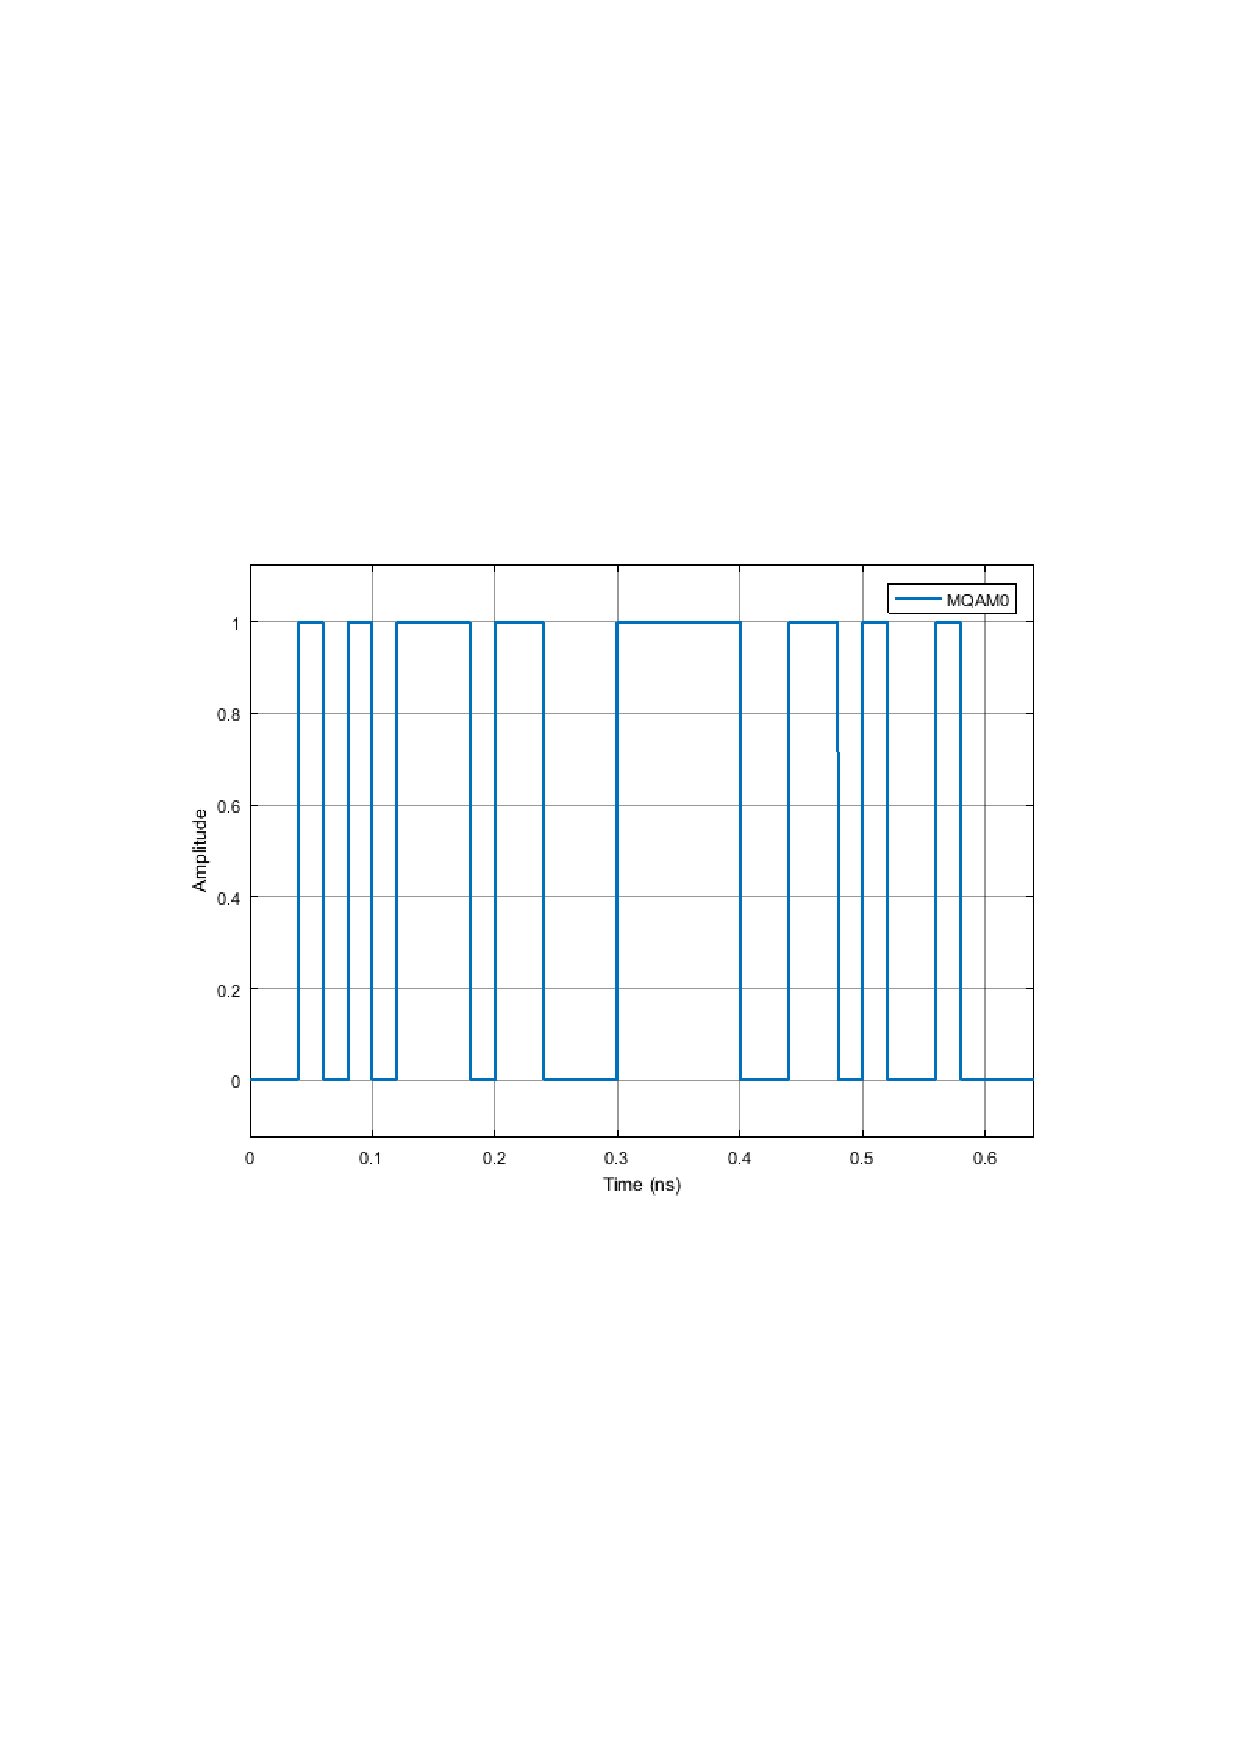
\includegraphics[width=\linewidth, trim= 0mm 95mm 0mm 95mm, clip]{binarystring.pdf}
\caption{Sent binary key.}
\label{fig:sentkey}
\end{figure}

\begin{figure}[H]
\centering
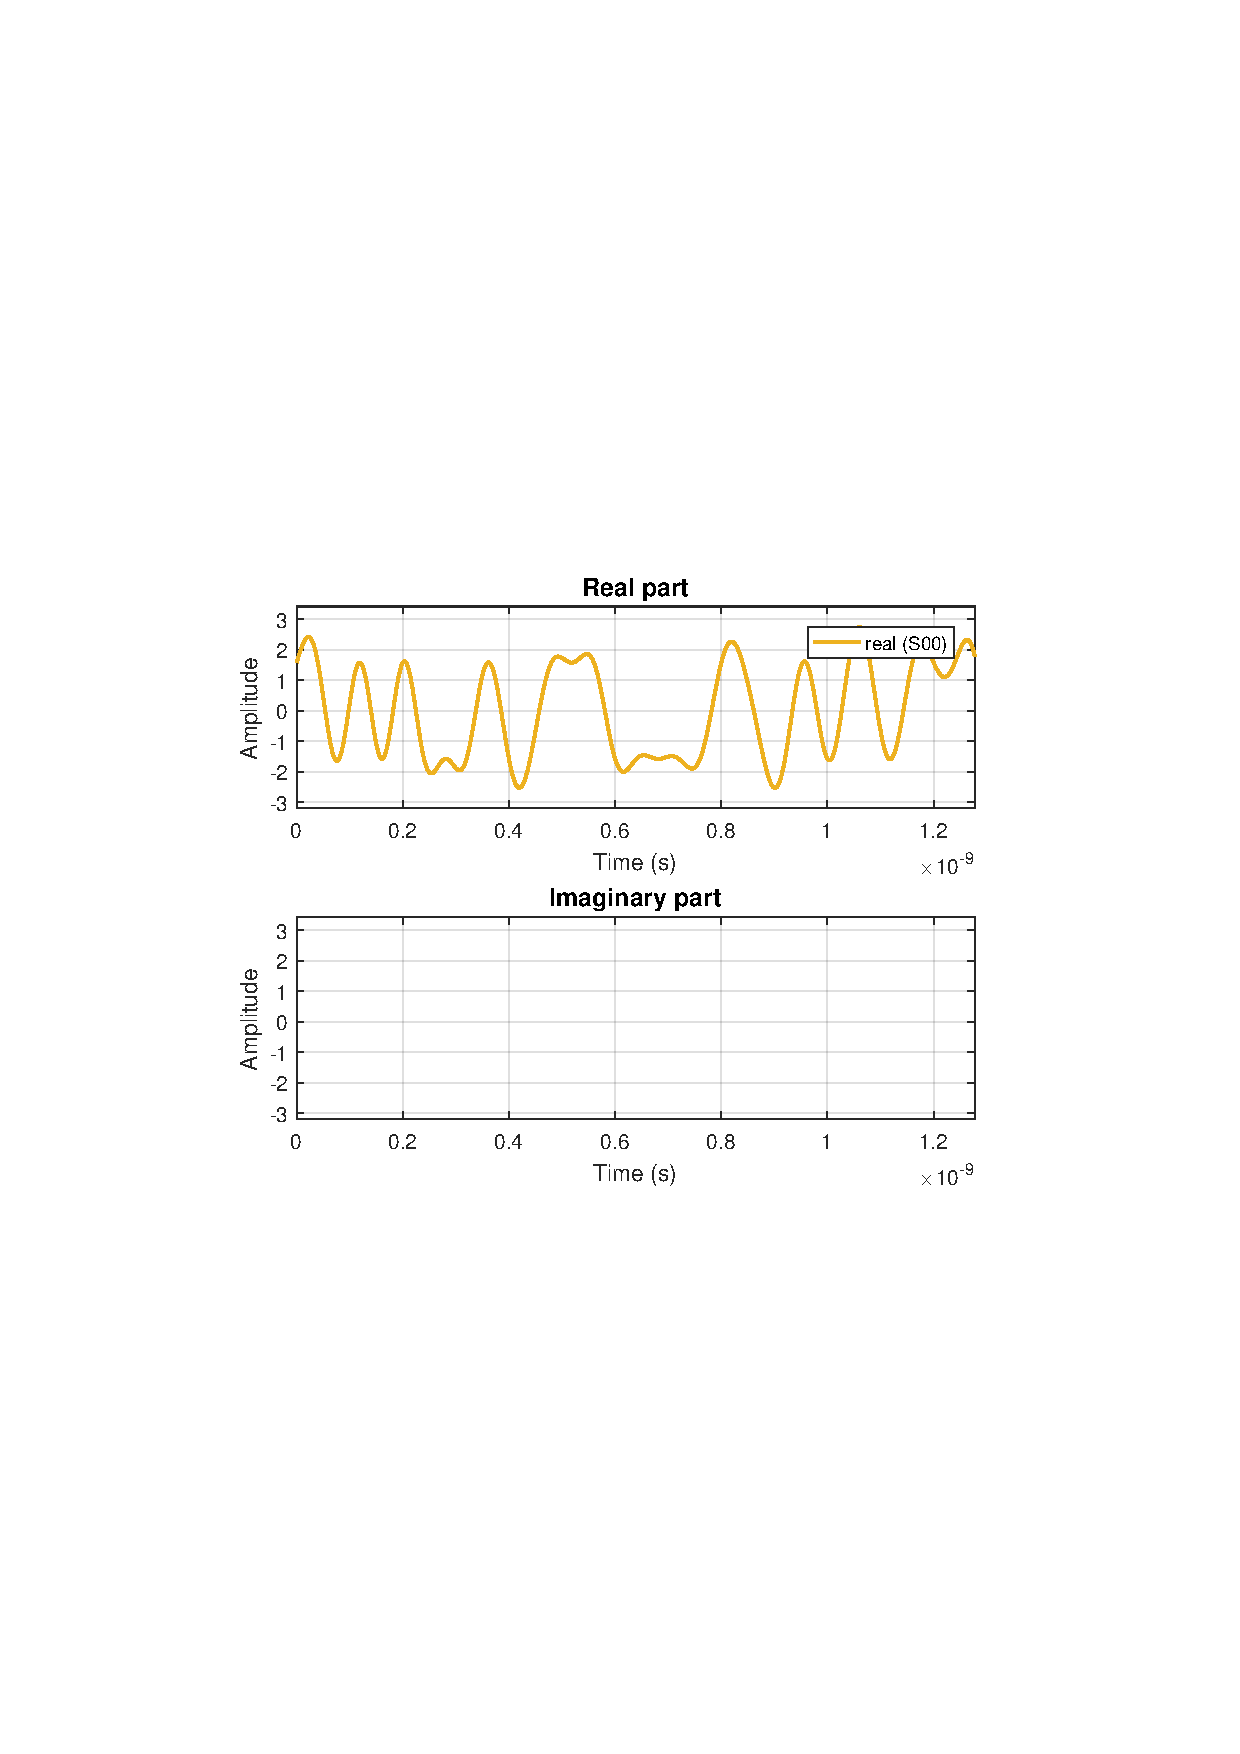
\includegraphics[width=\linewidth, trim= 0mm 95mm 0mm 95mm, clip]{sentsignal.pdf}
\caption{Sent signal.}
\label{fig:sentsig}
\end{figure}

\begin{figure}[H]
\centering
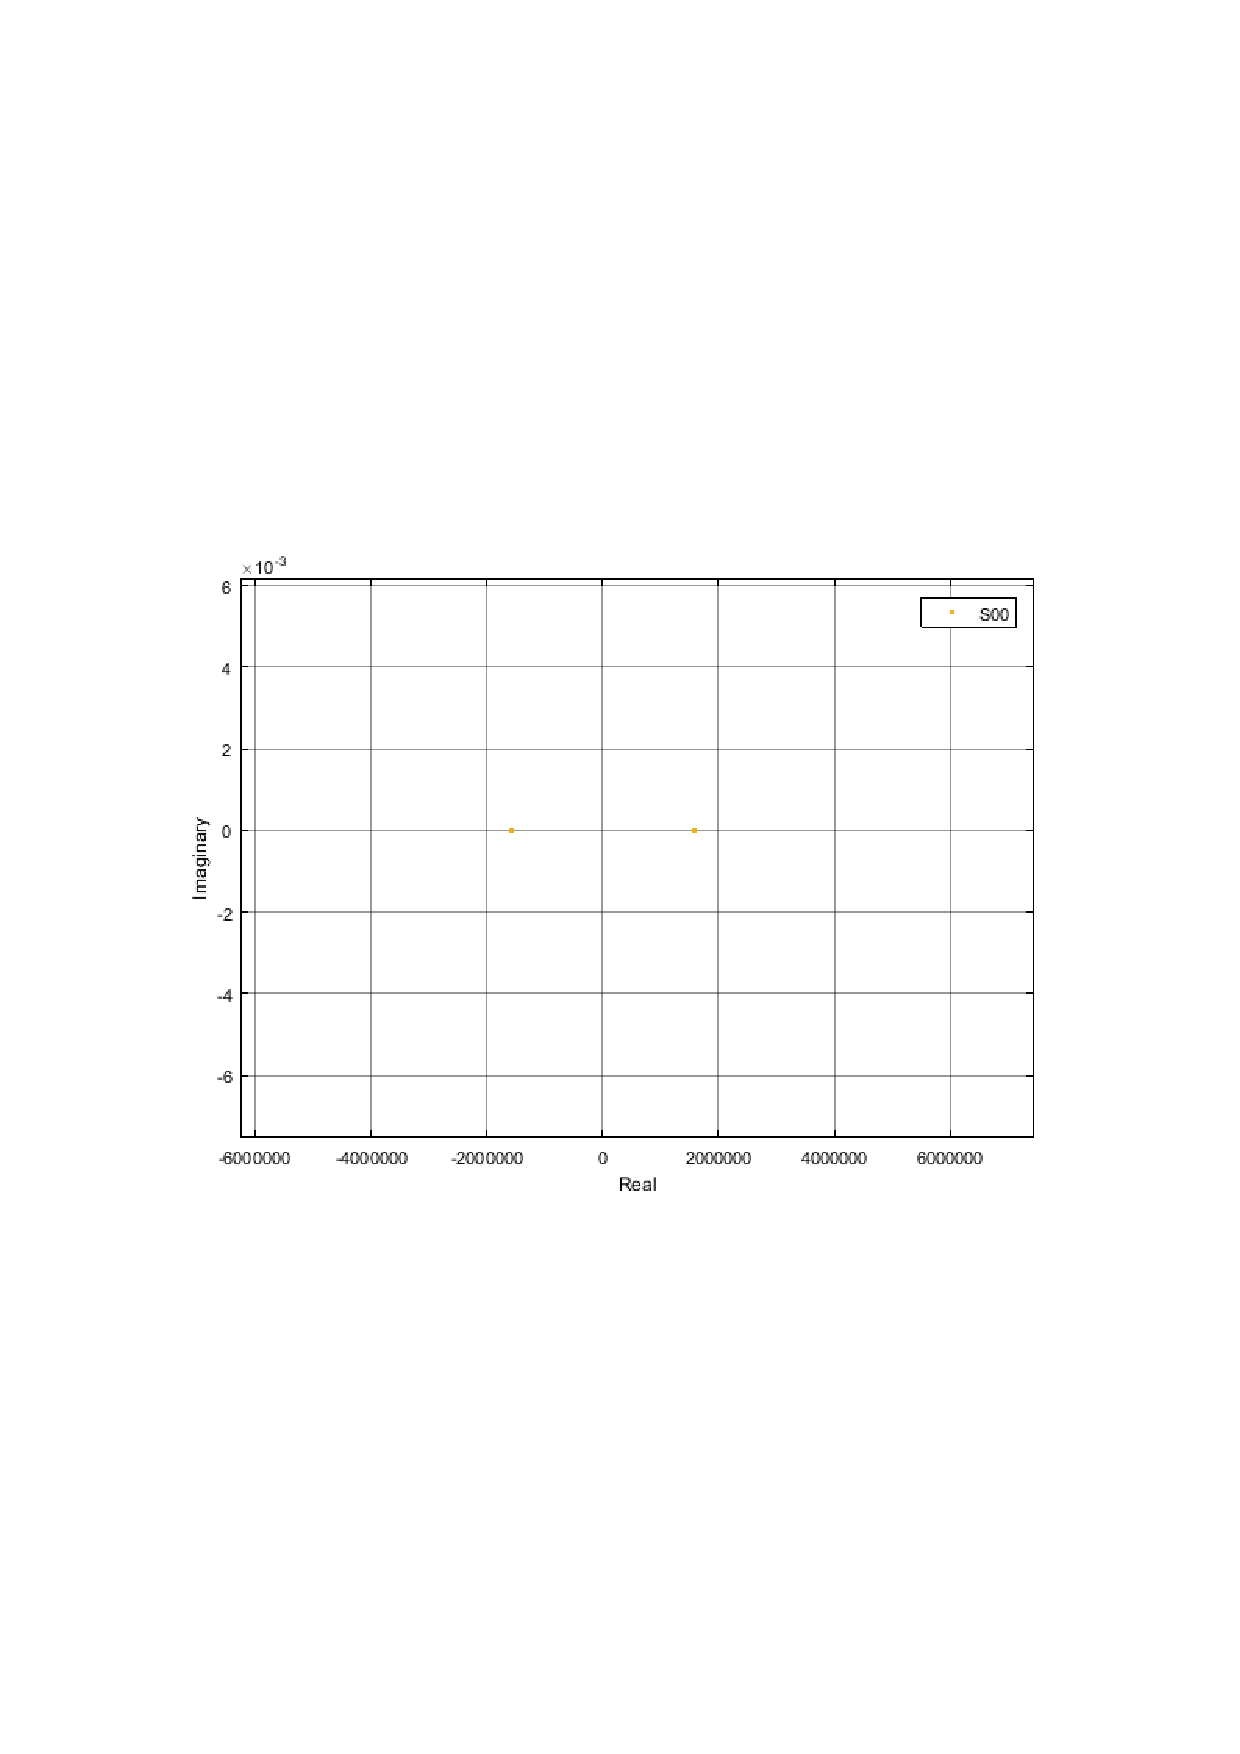
\includegraphics[width=\linewidth, trim= 0mm 95mm 0mm 95mm, clip]{constellation.pdf}
\caption{Constellation of the sent signal.}
\label{fig:constellation}
\end{figure}

Homodyne detection is then performed, using to that effect the local oscillator signal presented in Figure~\ref{fig:local}. Figures~\ref{fig:subtract}~and~\ref{fig:noisy} show the addition of noise to the signal.

\begin{figure}[H]
\centering
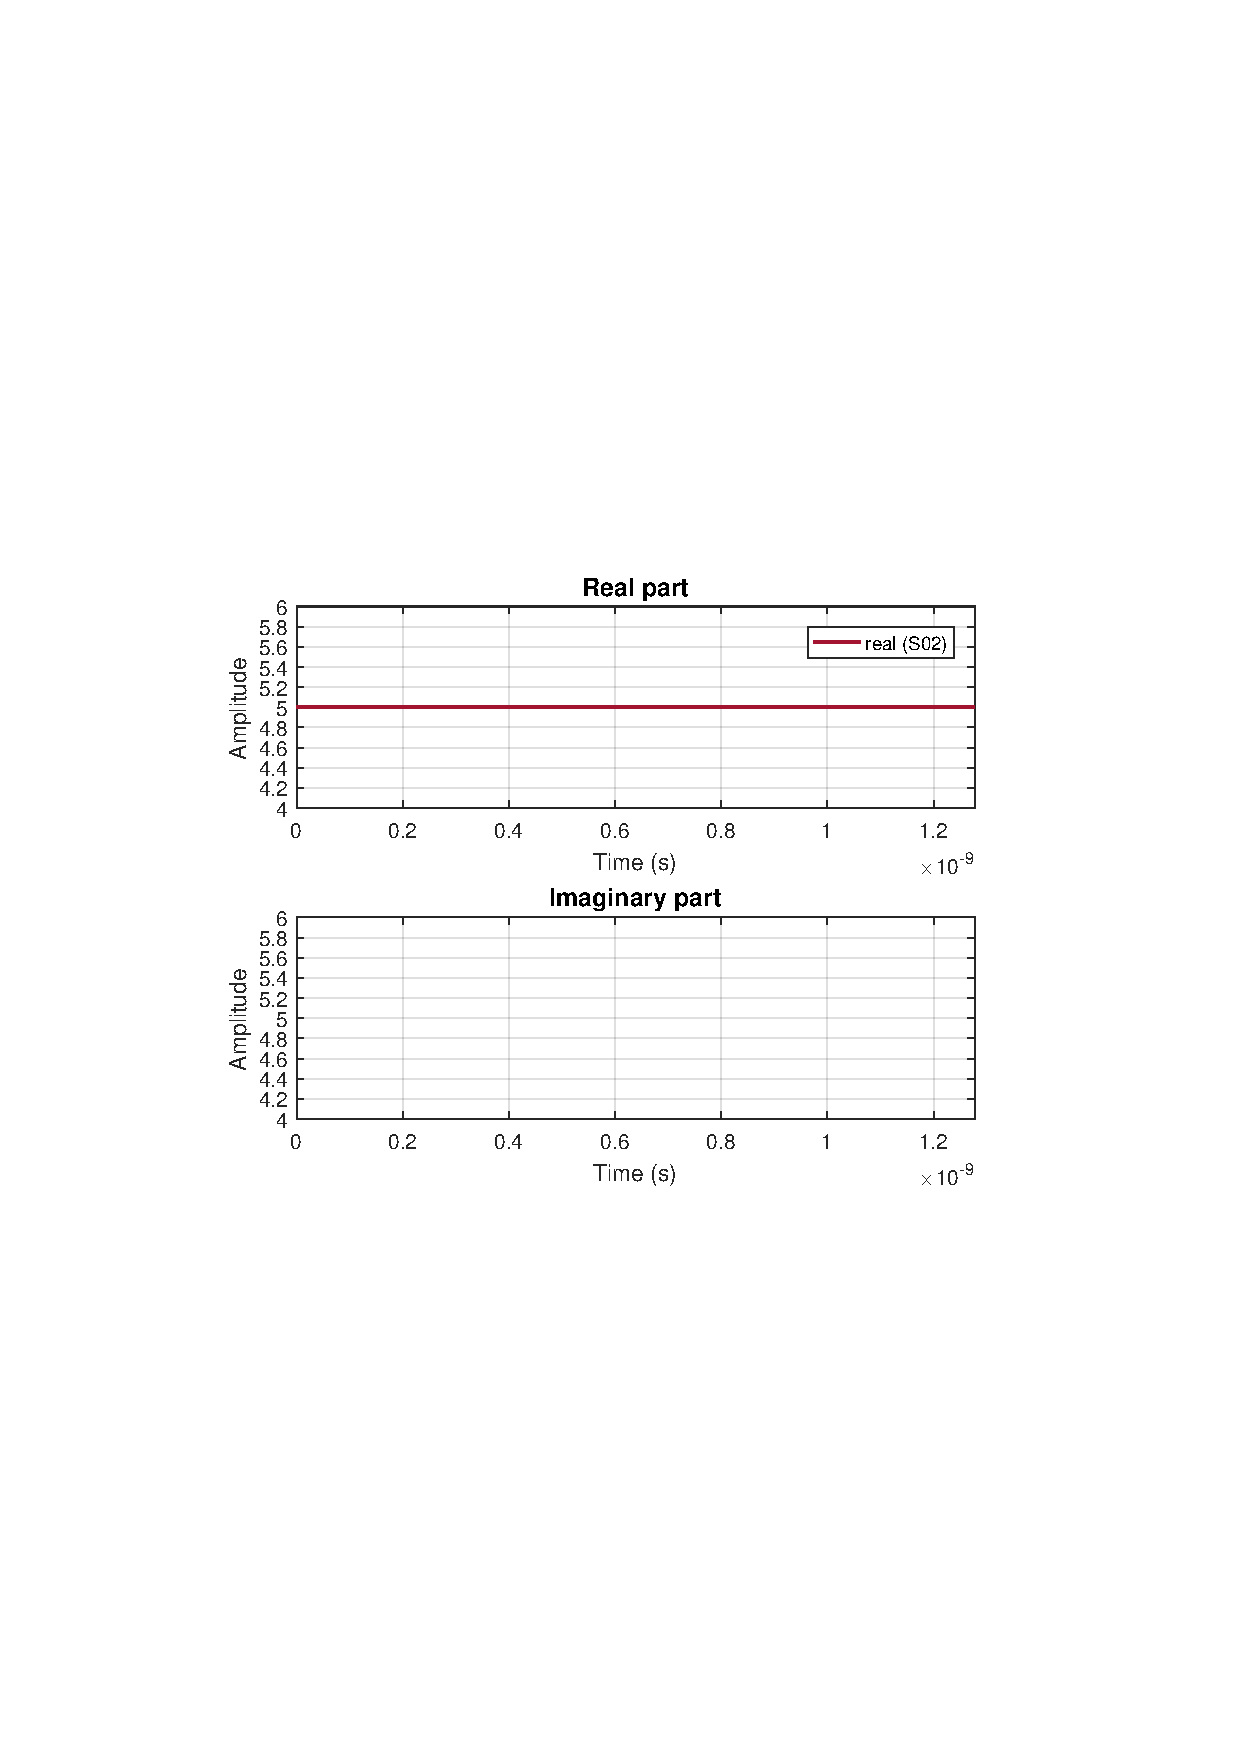
\includegraphics[width=\linewidth, trim= 0mm 95mm 0mm 95mm, clip]{localosc.pdf}
\caption{Homodyne receiver internal signal: local oscillator used for Homodyne detection.}
\label{fig:local}
\end{figure}

\begin{figure}[H]
\centering
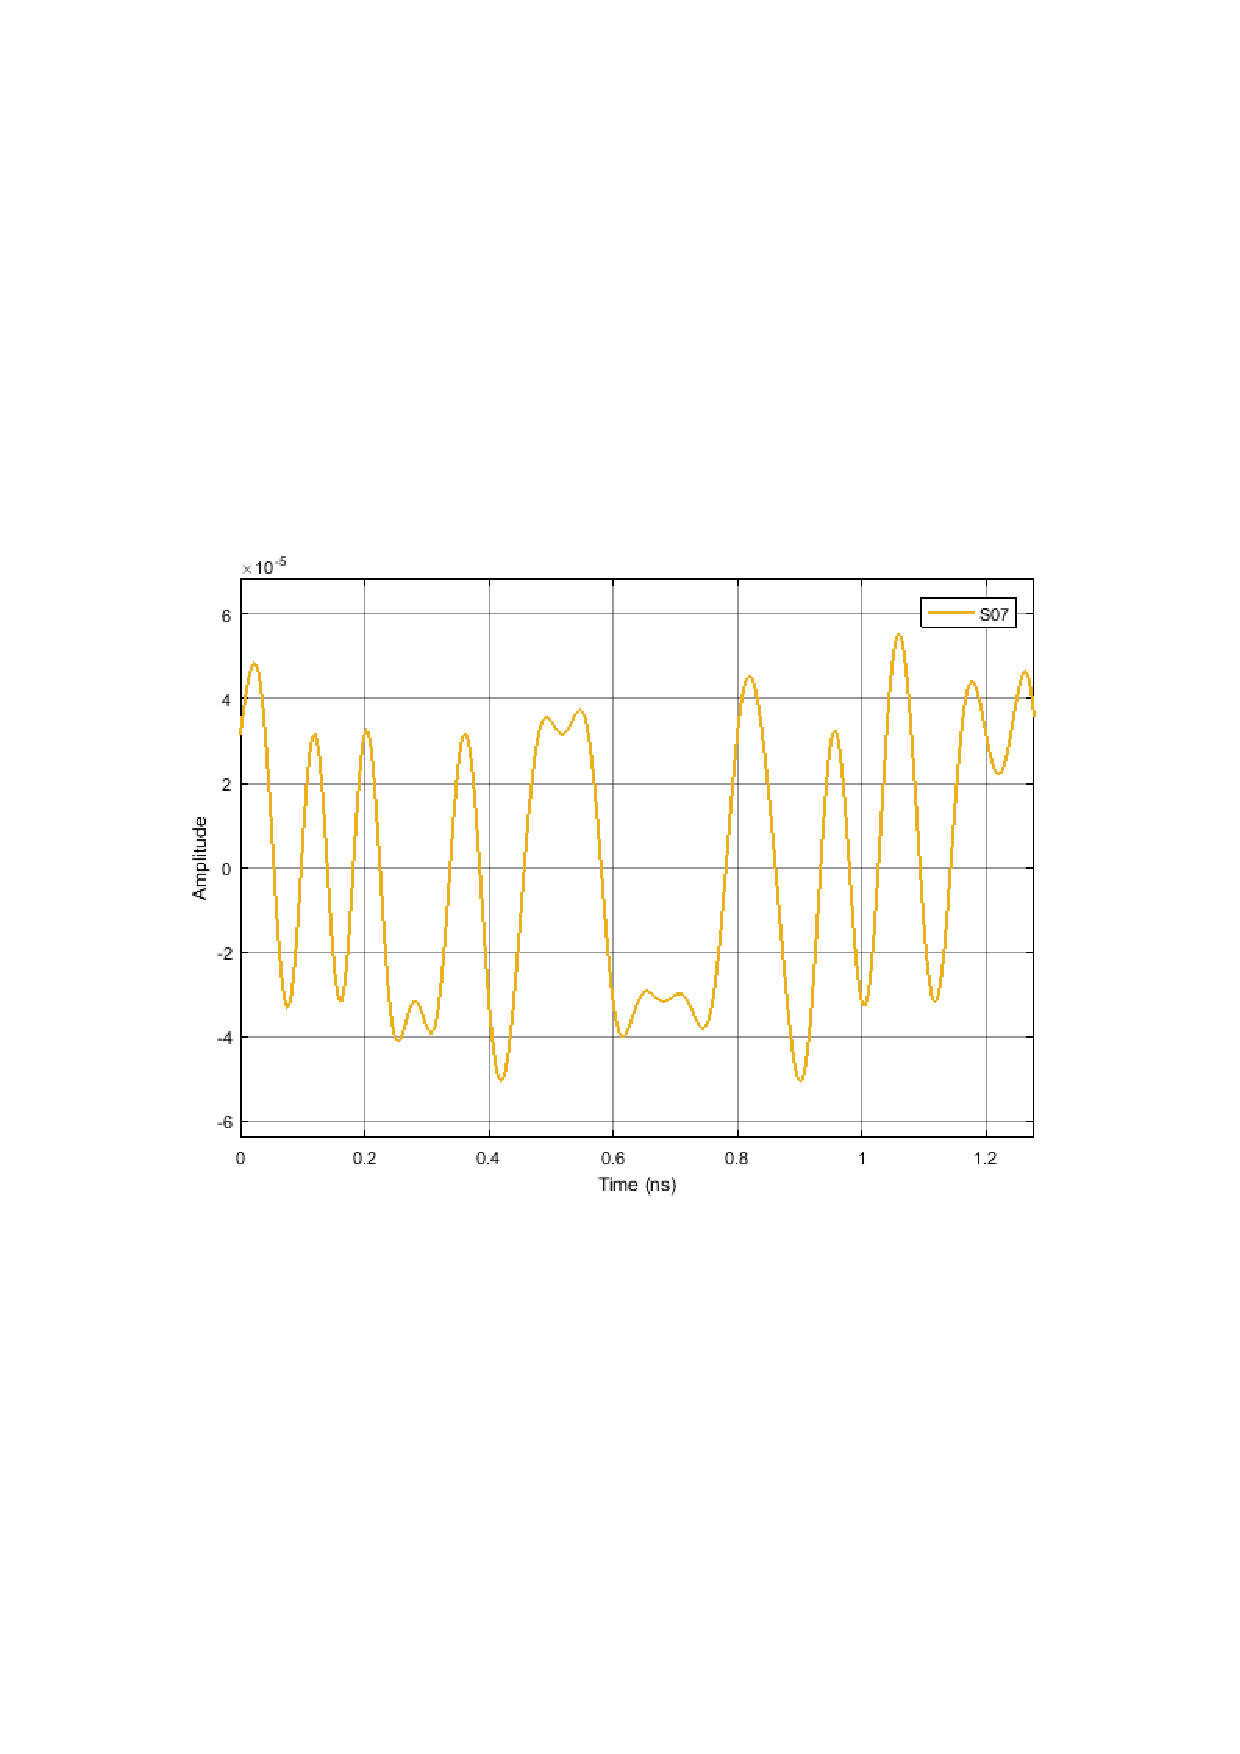
\includegraphics[width=\linewidth, trim= 0mm 95mm 0mm 95mm, clip]{subtract.pdf}
\caption{Homodyne receiver internal signal: subtraction of the signals outputted by the photodiodes.}
\label{fig:subtract}
\end{figure}

\begin{figure}[H]
\centering
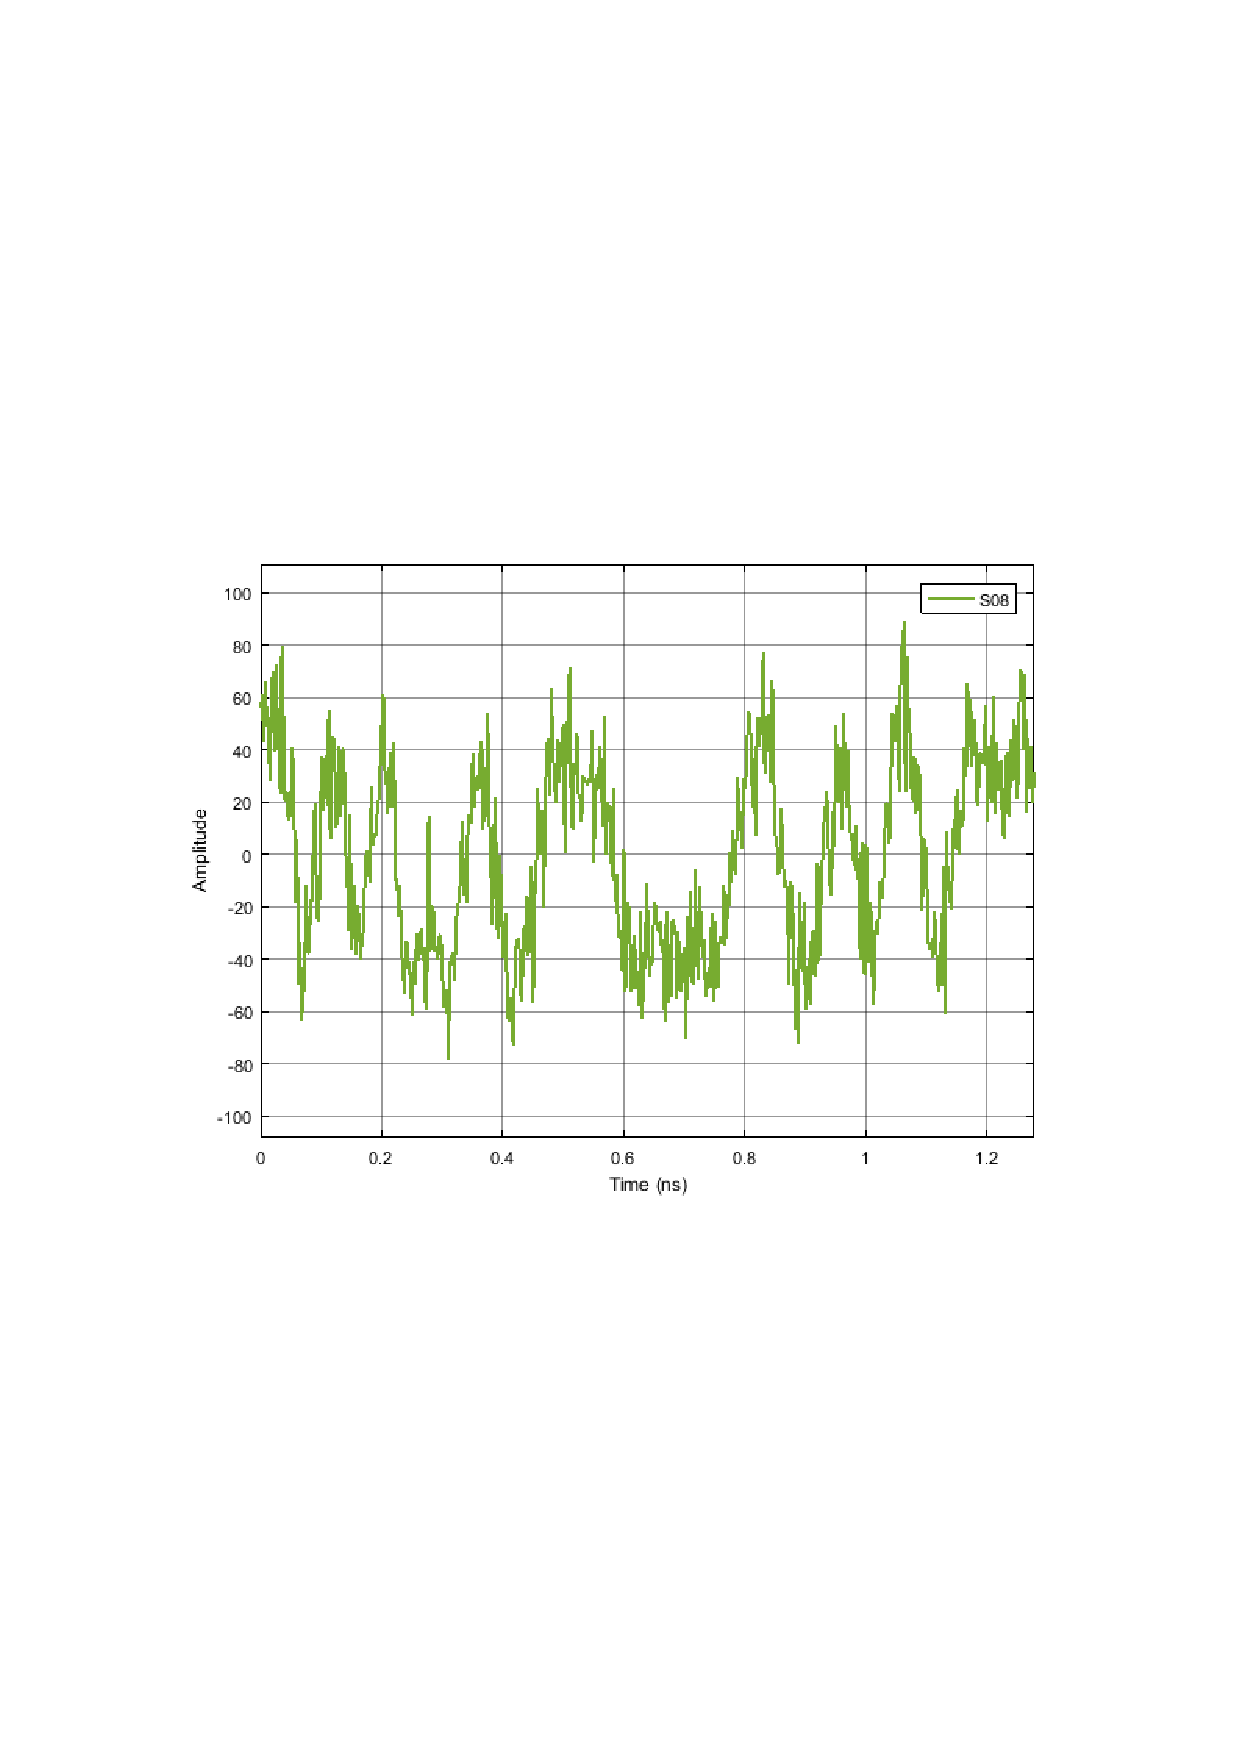
\includegraphics[width=\linewidth, trim= 0mm 95mm 0mm 95mm, clip]{noisy.pdf}
\caption{Homodyne receiver internal signal: amplification of the signal in Figure~\ref{fig:subtract} with added noise.}
\label{fig:noisy}
\end{figure}

The result of the homodyne detection is the binary string presented in~\ref{fig:decoded}, which is then compared to the original binary string by the BER block, which outputs the report presented in Figure~\ref{fig:ber}.

\begin{figure}[H]
\centering
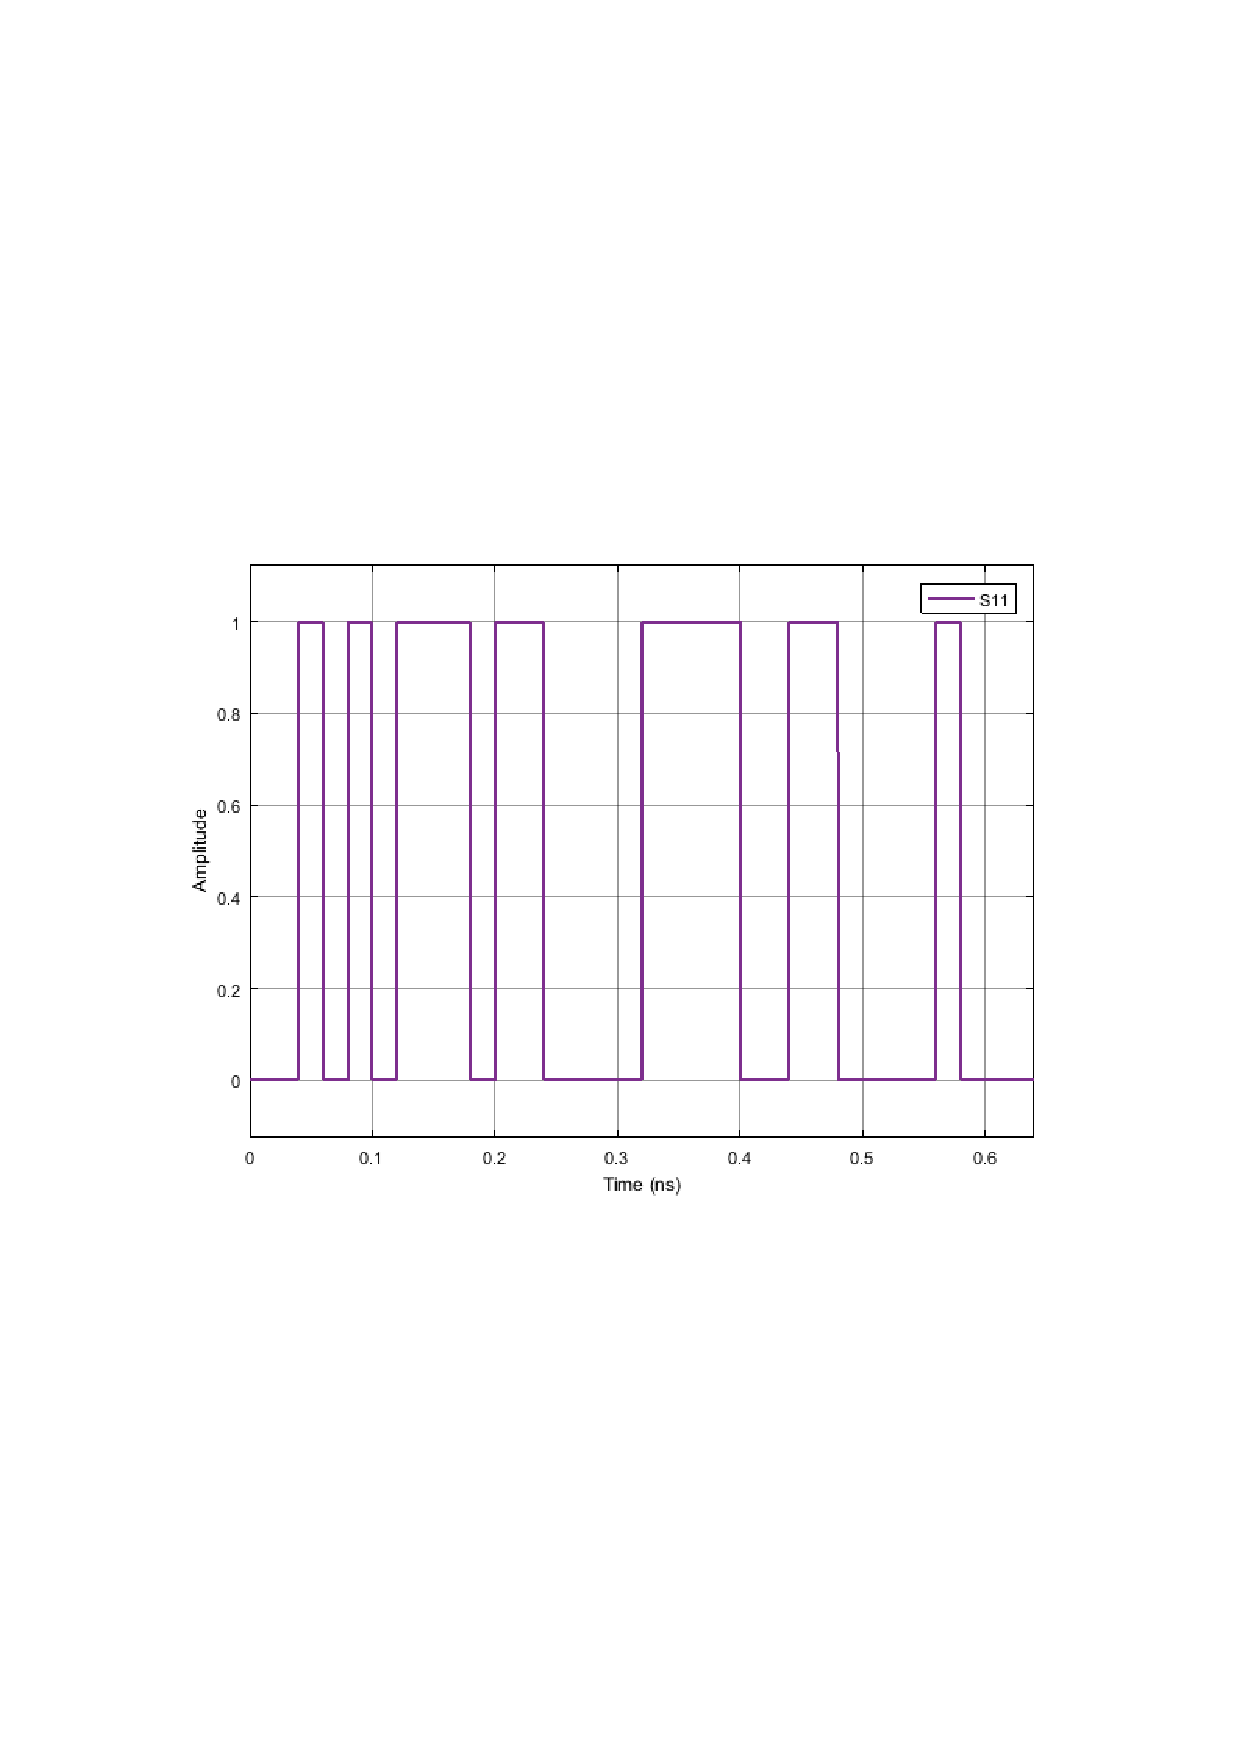
\includegraphics[width=\linewidth, trim= 0mm 95mm 0mm 95mm, clip]{decodedbinarystring.pdf}
\caption{Decoded binary string, output of the Homodyne receiver block.}
\label{fig:decoded}
\end{figure}

\begin{figure}[H]
\centering
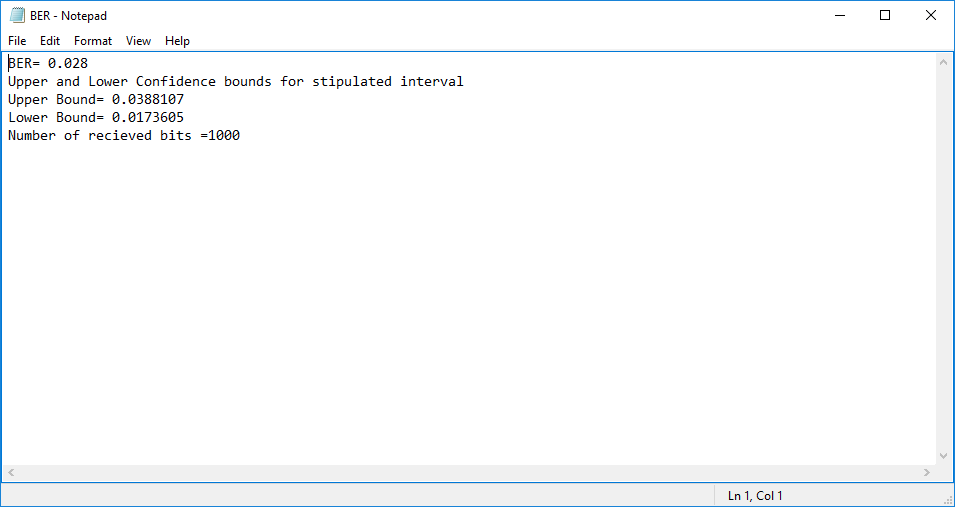
\includegraphics[width=\linewidth]{berreport.png}
\caption{Bit-Error-Rate report.}
\label{fig:ber}
\end{figure}

\pagebreak


\section{Block Description}

\subsection{MQAM Transmitter}
% subfile goes here

\subsection{Homodyne Receiver}
\subfile{../../lib/tex/homodyne_reciever}


\subsection{Bit Error Rate}
\subfile{../../lib/tex/ber}

\subsection{Local Oscillator}
\subfile{../../lib/tex/localoscillator}

\subsection{Beam Splitter}
\subfile{../../lib/tex/beamsplitter}

\subsection{Photodiode}
\subfile{../../lib/tex/photodiode}

\subsection{Subtractor}
\subfile{../../lib/tex/subtractor}

\subsection{Amplifier}
\subfile{../../lib/tex/amplifier}

\subsection{Discretizer}
\subfile{../../lib/tex/discretizer}

\subsection{Delayer}
\subfile{../../lib/tex/delayer}

\subsection{Bit Decider}
\subfile{../../lib/tex/decider}

\subsection{Bit Error Rate}
\subfile{../../lib/tex/ber}

\section{Known Problems}

\begin{itemize}
\item Homodyne Super-Block not functioning (problem in inputting signal into it)
\item MQAM Transmitter PDF needs to be written
\item 8 bits being lost of every signal
\item If the bit string length is larger than 512, this first 512 bits are lost
\item I don't think it is possible to declare nested subfiles, so I can't put the sub blocks into the homodyne receiver super block manual
\end{itemize}

\end{document}